%!TEX root = ../Thesis.tex
\chapter{Attitude dynamics: modelling and control}

\newcommand\scalemath[2]{\scalebox{#1}{\mbox{\ensuremath{\displaystyle #2}}}}

\textit{This chapter introduces the dynamics modelling principles used for this project, the reason for model-based approach and other modelling decisions, as well as the control system as following the previous chapters}

\section{Model-based design approach}

The motivation for model-based design of the controller is that this can be useful on a system even before the physical system exists, as it is the case for the Spica rocket. Model-based tuned controller can be more efficient, more precise and less error prone, therefore requiring less controller corrections needed, which translates into more precise movements and conservation of energy and resources. Model-based also implies that scalability towards the rocket is inherent. 

In this sense it is useful to have an abstraction of the physical system, which can be very complex and would be overwhelming to deal with all its structural parts. It is easier to make changes but also a model-based approach allows the controller to be more precise and suited for that particular type of system.

The approach chosen in this thesis is derivation of the dynamics model from first principles. This approach provides understanding of all aspects of the model - as opposed to choosing system identification from empirical data. This would run the risk of having an oversimplified model. The model is then validated through empirical data - from tests - and also as a means to determine its parameters for accuracy of the model. The model’s aim is not a high degree of accuracy but having a reliable starting point. This model would be used for analysis for the  system as opposed to design.

Having a model helps map more precisely the input to output and to see how the different parameters (inertia etc) affect the response of the system. The model does not include an important part: the point of saturation of the actuators of components. Another simplification consists of the model assuming its parameters are time invariant. They may in fact change with temperature etc. It is necessary to take into consideration actuator delays and other interactions between the links of the rocket; it is not a static system, it’s dynamic: it will take time to react. It varies with time, depending on initial conditions and past inputs. 

The more complex model which includes the non-linear, time-varying parameters can be tested through simulation, achieving higher accuracy. Simulation allows for varying different parameters and observing their response in real time. Since there is interest in the transient response of the system as opposed to purely steady-state response, the system will be modeled as a dynamic system.

\section{Model: kinematics and dynamics - Newton-Euler approach for rigid multi-body systems}


The aim of this section is to analyze the kinematic and dynamic behavior of the dual propeller system described above. For this project, the approach is Newton-Euler for multi-body systems, where bodies are separated at the joints, each body considered an individual unit, considered rigid bodies. This modelling strategy used in this project section was introduced in (Santos, 2003) \cite{santos2001dinamica}. 

Newton-Euler was preferred as opposed to Lagrange due to the focus being on understanding the interplay of forces as opposed to the energy in the mechanical system, relevant for the drone as well as for the rocket. The mechanical system consists of a static structure (drone frame, propellers) and three moving rigid bodies, approached in 2D. The moving bodies form the servo-rudder system, with three bodies and one degree of freedom, the servo arm angle. 

\begin{figure}[h!]
  \centering
  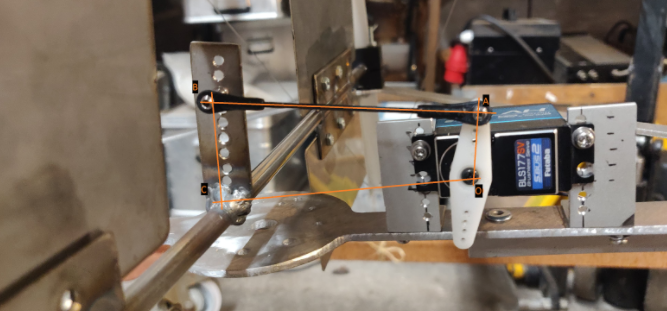
\includegraphics[scale=0.8]{graphics/ConstraintServoPic.png}
  \caption{The servo-rudder mechanical system}
  \label{fig:Servo-rudder mechanical system}
\end{figure}

\textit{Nomenclature}
 
\begin{center}
\begin{tabular}{ | m{5em} | m{6cm}|  } 
\hline
Symbol & Meaning \\ 
\hline
\textit{a} & absolute acceleration \\
\hline
\textit{t} & time \\ 
\hline
\textit{m} & mass \\ 
\hline
\textit{g} & acceleration due to gravity  \\
\hline
$\theta$ & angular displacement (scalar) \\ 
\hline
$\dot{\theta}$ & angular velocity (scalar) \\ 
\hline
$\ddot{\theta}$ & angular acceleration (scalar) \\
\hline
$ {\omega} $  & angular velocity (vector) \\ 
\hline
\textit{CM} & center of mass \\ 
\hline
\textit{r} & position vector \\ 
\hline
\textit{F} & force \\ 
\hline
${B_x}$& body number x \\ 
\hline
\textit{T}& transformation matrix \\ 
\hline
\textit{I} & moment of inertia \\ 
\hline
\end{tabular}
\end{center}
 
 

\textit{Parameters List }
 
\begin{tabular}{ |p{1.5cm}||p{7 cm}|p{3cm}|p{2cm}|  }
 \hline
 \multicolumn{4}{|c|}{Parameters List} \\
 \hline
 Symbol & Parameter &  Quantity & Units\\
 \hline
 $m_0 $  & mass body 0 & 2.75 & kg\\
$m_1 $ & mass body 1 & 0.05 & kg\\
$m_2 $ & mass body 2 & 0.00005 & kg\\
$m_3 $ & mass body 3 & 0.54 & kg\\
$I_{zz0} $ & rotational inertia about Z axis body 0 & 0.1 & kg\times $m^2$\\
$I_{zz1}$ & rotational inertia about Z axis body 1 & 0.625 & kg\times $m^2$\\
$I_{zz2}$ & rotational inertia about Z axis body 2 & 0.2408 \times $10^{-25}$ & kg\times $m^2$\\
$I_{zz3}$ & rotational inertia about Z axis body 3 & 0.0022 & kg\times $m^2$\\
$Fprop$ & thrust force & 30 & N\\
g & acceleration due to gravity & 9.8 & m/s^2\\
 \hline
\end{tabular}


\begin{figure}[h!]
  \centering
  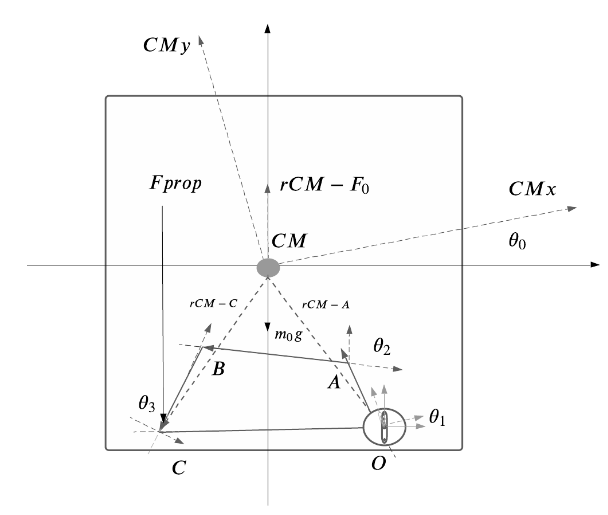
\includegraphics[scale=0.8]{graphics/DroneFBD.png}
  \caption{Free-body diagram of the drone body frame}
  \label{fig:Free-body diagram of the drone body frame}
\end{figure}



The prototype is modelled as a fixed-axis rotation body. The dynamical equations of motion and the dynamic reaction forces are derived. Translational equations are written in the inertial frame, rotational equations are written in the moving body frame.Defining the inertial\textbf{ (I) }and the moving coordinate systems for the bodies \textbf{(B0, B1, B2, B3) }in this mechanism and the free-body diagram of the mechanical system defining each of the three bodies and the interplay of reaction forces (Santos, 2003) \cite{santos2001dinamica}:

\subsection{Reference frames}


\textbf{I} - inertial X, Y, Z;\textbf{ i, j, k}

\textbf{B0}- moving body 0:\textbf{ i0, j0, k0 }

\textbf{B1}- moving body 1:\textbf{ i1, j1, k1 }

\textbf{B2-} moving body 2: \textbf{i2, j2, k2}

\textbf{B3}- moving body 3:\textbf{ i3, j3, k3 }






\begin{figure}[h!]
  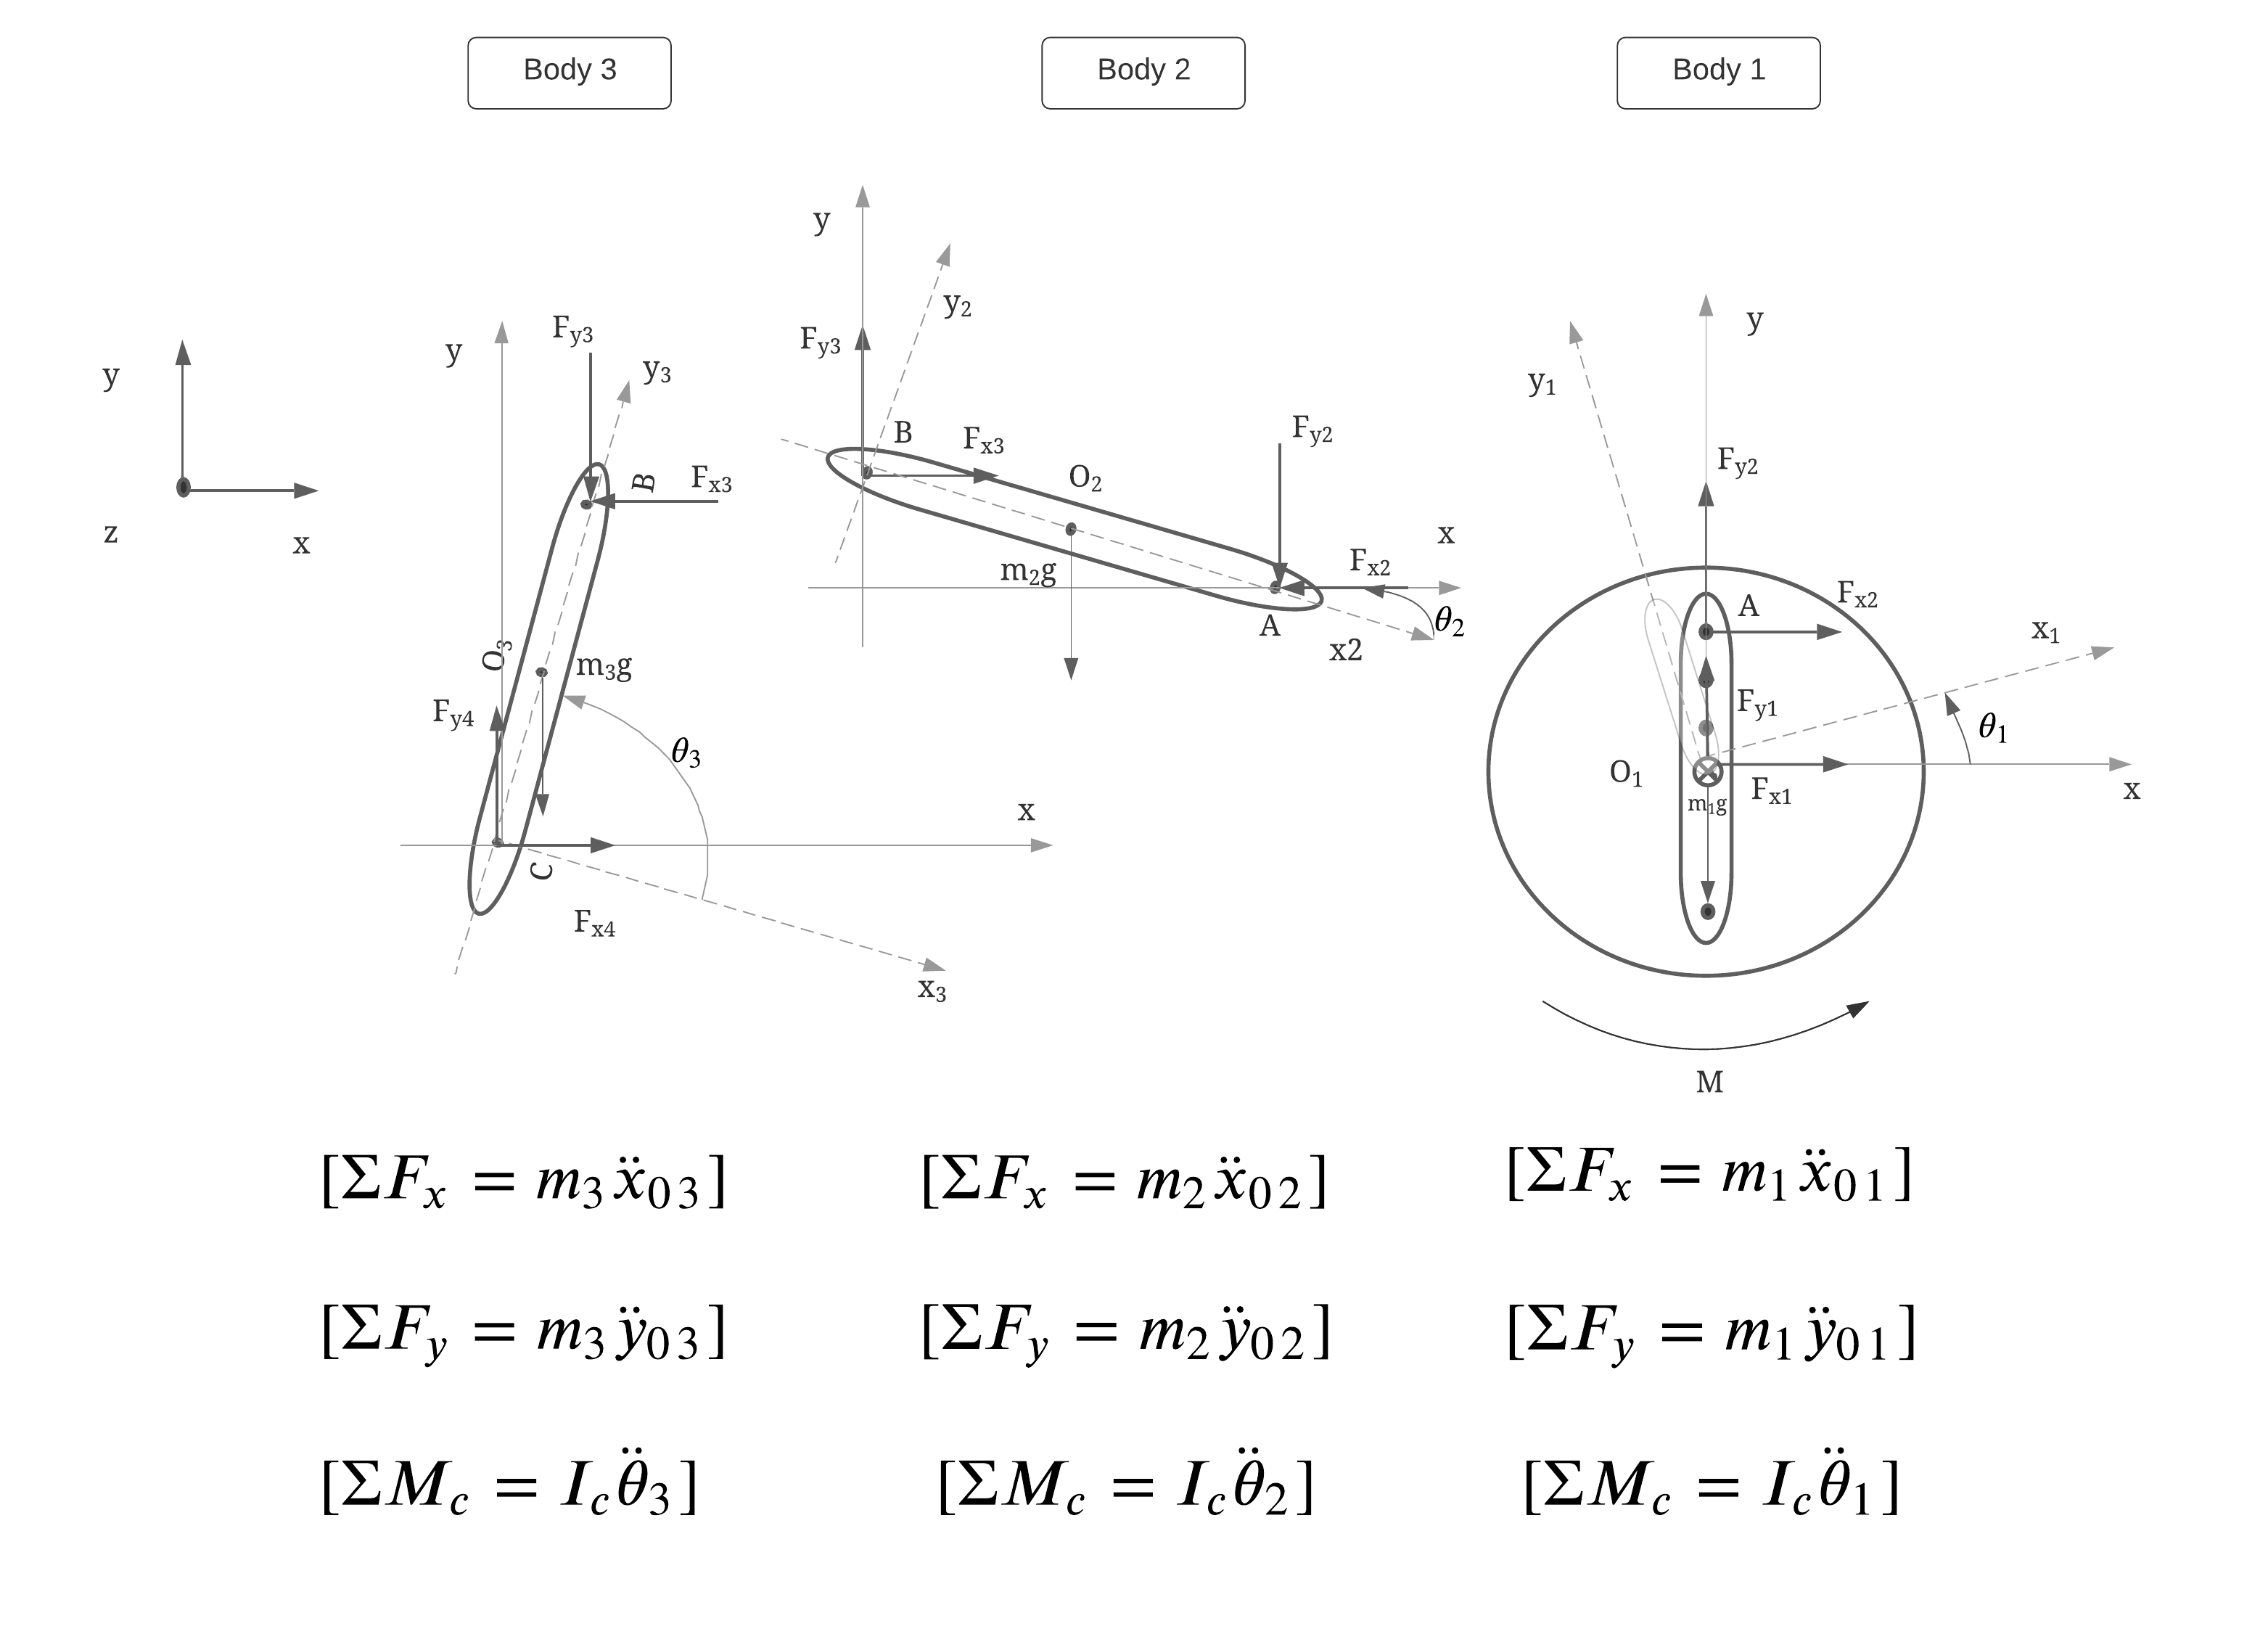
\includegraphics[scale=0.6]{graphics/Servo-Rudder2.png}
  \caption{Free-body diagram of the servo-rudder mechanical system}
  \label{fig:free-body diagram of the servo-rudder mechanical system}
\end{figure}


Defining the transformation matrix from the inertial coordinate system \textbf{(I)} to body coordinate systems \textbf{(B1, B2, B3) } \cite{santos2001dinamica}.

\begin{equation}\label{rotmat}
	T_{\theta} = \left[ \begin {array}{ccc} \cos\,\theta&\sin\,\theta&0
\\ \noalign{\medskip}-\sin\,\theta&\cos\,\theta&0
\\ \noalign{\medskip}0&0&1\end {array} \right]
\end{equation}

Defining the transformation from inertial frame to body frame as

\begin{equation}\label{i_to_B}
_{B}{r} = T_{\theta}  {_I}{r}
\end{equation}

and from body frame to inertial frame as

\begin{equation}\label{b_to_I}
_{I}{r} = T_{\theta}^T {_B }{r}
\end{equation}


Writing the displacement vectors for the each of the three bodies of the mechanism in the body frame and the distance from point C to O, closing the constraint equation, in the inertial frame


\begin{equation} \label{disp_vec1}
 _B{_1}\vec{r}_{OA} = \left[ \begin {array}{c} 0\\ \noalign{\medskip} 0.02
\\ \noalign{\medskip}0\end {array} \right ]   [m]
\end{equation}
\begin{equation}\label{disp_vec2}
 _B{_2}\vec{r}_{AB} = \left[ \begin {array}{c} - 0.08\\ \noalign{\medskip}0
\\ \noalign{\medskip}0\end {array} \right] [m]
\end{equation}
\begin{equation}\label{disp_vec3}
_B{_3}\vec{r}_{BC} =  \left[ \begin {array}{c} 0\\ \noalign{\medskip}- 0.036
\\ \noalign{\medskip}0\end {array} \right]  [m]
\end{equation}
\begin{equation}\label{disp_vec4}
_I\vec{r}_{CO} =  \left[ \begin {array}{c}  0.078\\ \noalign{\medskip}0
\\ \noalign{\medskip}0\end {array} \right] [m]
\end{equation}

The individual bodies are presented with their properties: mass, mass moment of inertia and displacement vector from the center of mass. The bodies are thin, with negligible thickness and their mass moment of inertia was calculated with the bodies modeled as rods.

\begin{wrapfigure}{l}{0.25\textwidth}
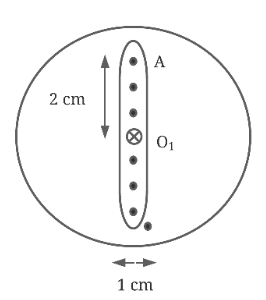
\includegraphics[width=0.9\linewidth]{graphics/body1.png}
\caption{Servo}
\label{fig:wrapfig}
\end{wrapfigure}

Body 1: Servo arm, rotating about its center pivot. The servo arm has a length of 0.02 m from pivot point to end of servo arm, coinciding with center of mass of the body, mass = 0.003 kg and a calculated mass moment of inertia around Z axis of Izz1 = 6.25e-7 kg/m2. The servo arm has negligible thickness.

\begin{wrapfigure}{l}{0.3\textwidth}
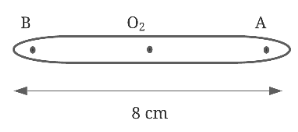
\includegraphics[width=0.9\linewidth]{graphics/Body3.png}
\caption{Link}
\label{fig:wrapfig}
\end{wrapfigure}

Body 2 has mass of m = 0.001 kg and mass moment of inertia around Z axis of Izz2 = 2.408333e-15  kg/m2. The center of mass of the body AB is at the middle of the length between the points. 

The link has negligible thickness.

\begin{wrapfigure}{l}{0.3\textwidth}
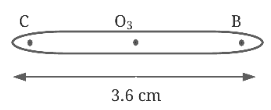
\includegraphics[width=0.9\linewidth]{graphics/Body2.png}
\caption{Rudder arm}
\label{fig:wrapfig}
\end{wrapfigure}

Body 3: rudder has a mass m = 0.54 kg and mass moment of inertia around Z axis of Izz3 = 0.0022 kg/m2. 
It has its center of mass at the point of contact with the rudder (labeled C)
 
 Further the connection points between the three bodies are shown, forming the constraint equation. 

\begin{equation}\label{constraint}
_I\vec{r}_{0A} + {_I}\vec{r}_{AB}+{_I}\vec{r}_{BC}+{_I}\vec{r}_{C0}=0
\end{equation}

 
 \begin{figure}[h!]
  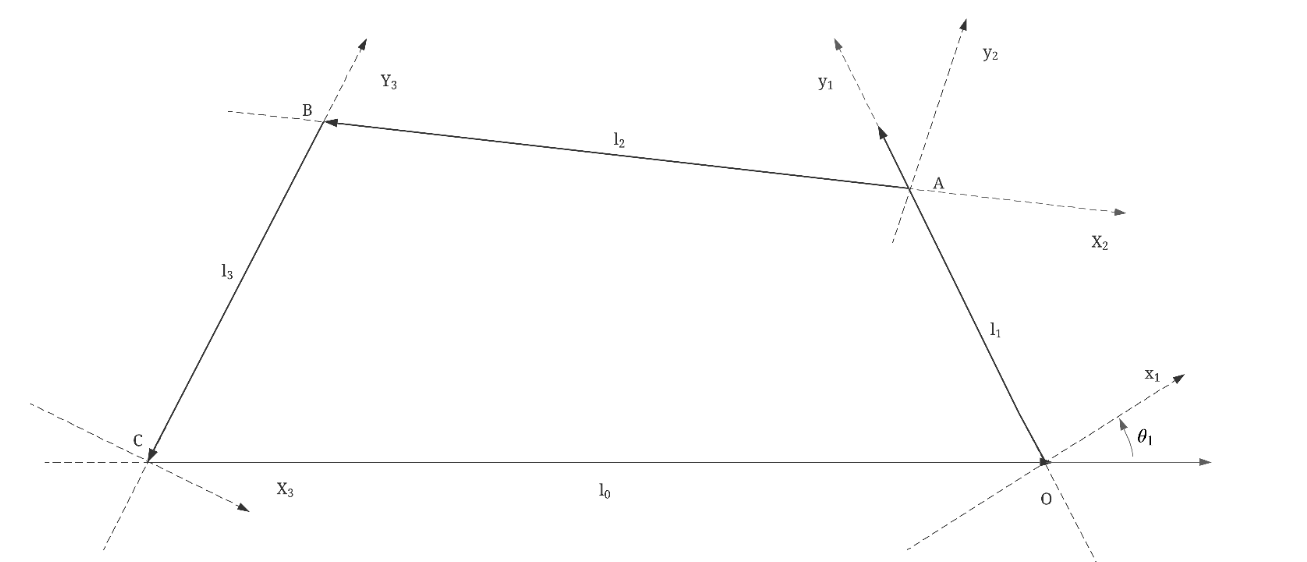
\includegraphics[scale=0.55]{graphics/ConstraintFigure.png}
  \caption{Constraint Figure}
  \label{fig:Constraint Figure}
\end{figure}
 
The constraint equation is formed by having the displacement vectors transformed from body frame to inertial frame and equaled to 0. 

\begin{equation}\label{constraintlong}
_I\vec{r}_{0A} + {_I}\vec{r}_{AB}+{_I}\vec{r}_{BC}+{_I}\vec{r}_{C0}=0 \\
=> \\T_{\theta _1}^T {_B}\vec{r}_{0A} + T_{\theta _2}^T {_B}\vec{r}_{AB} + T_{\theta _3}^T {_B}\vec{r}_{BC} + {_I}\vec{r}_{C0}=0 
\end{equation}

Therefore, results the following constraint equation in inertial reference frame.

\begin{equation}\label{constvector}
 \left[ \begin {array}{c} - 0.02\,\sin\,\theta_{1}
\\ \noalign{\medskip} 0.02\,\cos\,\theta_{1}\\ \noalign{\medskip} 0.0
\end {array} \right] 
+
 \left[ \begin {array}{c} - 0.08\,\cos\,\theta_{2}
\\ \noalign{\medskip}- 0.08\,\sin\,\theta_{2}\\ \noalign{\medskip}
 0.0\end {array} \right] 
+
 \left[ \begin {array}{c}  0.036\,\sin\,\theta_{3}
\\ \noalign{\medskip}- 0.036\,\cos\,\theta_{3}\\ \noalign{\medskip}
 0.0\end {array} \right]
+ \left[ \begin {array}{c}  0.078\\ \noalign{\medskip}0
\\ \noalign{\medskip}0\end {array} \right] 
= \left[ \begin {array}{c} 0\\ \noalign{\medskip}0\\ \noalign{\medskip}0
\end {array} \right] 
\end{equation}

The coordinate $\theta_1 $ [rad] is the master coordinate which describes the servo’s angular position (body 1).
$\theta_2 $[rad] and $\theta_3 $[rad] are “slave” coordinates, responsible for describing the angular position of bodies 2 and 3 depending on the motion of body 1, therefore $\theta_2 $ and $\theta_3 $ are described as a function of $\theta_1 $. Results a system composed of two nonlinear algebraic equations which will be numerically solved through a method capable of solving for roots of non-linear equations. In this project, the Newton-Raphson method has been used to iteratively arrive at the roots, describing the two slave coordinates. By differentiating the constraint equation (\ref{constraint}), results the angular velocity of the bodies. By using Cramer's rule, results the angular velocities $\dot{\theta}{_2}$ and $\dot{\theta}{_3}$ as a function of the servo angular rate $\dot{\theta}{_1}$

\begin{equation}\label{dtheta2}
\dot{\theta}{_2} =	{\frac { 0.00072\, \left( {\frac {\rm d}{{\rm d}t}}\theta_{{1}}
 \left( t \right)  \right) \cos \left( \theta_{{1}} \left( t \right) 
 \right) \sin \left( \theta_{{3}} \left( t \right)  \right) - 0.00072
\,\cos \left( \theta_{{3}} \left( t \right)  \right)  \left( {\frac 
{\rm d}{{\rm d}t}}\theta_{{1}} \left( t \right)  \right) \sin \left( 
\theta_{{1}} \left( t \right)  \right) }{ 0.00288\,\sin \left( \theta_
{{2}} \left( t \right)  \right) \sin \left( \theta_{{3}} \left( t
 \right)  \right) + 0.00288\,\cos \left( \theta_{{3}} \left( t
 \right)  \right) \cos \left( \theta_{{2}} \left( t \right)  \right) }
}
\end{equation}

\begin{equation}\label{dtheta3}
\dot{\theta}{_3} =	{\frac { 0.0016\,\sin \left( \theta_{{2}} \left( t \right)  \right) 
 \left( {\frac {\rm d}{{\rm d}t}}\theta_{{1}} \left( t \right) 
 \right) \sin \left( \theta_{{1}} \left( t \right)  \right) + 0.0016\,
 \left( {\frac {\rm d}{{\rm d}t}}\theta_{{1}} \left( t \right) 
 \right) \cos \left( \theta_{{1}} \left( t \right)  \right) \cos
 \left( \theta_{{2}} \left( t \right)  \right) }{ 0.00288\,\sin
 \left( \theta_{{2}} \left( t \right)  \right) \sin \left( \theta_{{3}
} \left( t \right)  \right) + 0.00288\,\cos \left( \theta_{{3}}
 \left( t \right)  \right) \cos \left( \theta_{{2}} \left( t \right) 
 \right) }}
\end{equation}

Differentiating the constraint equation (\ref{constraint}) twice, results the angular acceleration of bodies of bodies 2 and 3. By using Cramer's rule, results the angular acceleration $\ddot{\theta}{_2}$ and $\ddot{\theta}{_3}$ as a function of the servo angular acceleration $\ddot{\theta}{_1}$. The equations are larger than can be displayed here, therefore they are available in scaled down form in the appendix,  (\ref{ddtheta2}) and  (\ref{ddtheta3}).

\subsection{Absolute linear acceleration}

The next step is calculating the absolute linear acceleration vectors of the center of mass of the moving bodies. The absolute linear acceleration at the center of mass of each body is composed of normal and tangential acceleration. 

The absolute velocity vector is defined as the derivative in time of the position vector and the absolute acceleration vector is the derivative in time of the position vector.

The calculations are done in inertial frame, in order to obtain the absolute position vectors and their absolute  derivatives, without losing information. \cite{santos2001dinamica}.

\textbf{Body 0 - UAV frame}

\begin{equation}\label{aabody0}
{_B}_{0}\vec{a}_{01} = {_B}_{0}\vec{\omega}_{0}\times \,({_B}_{0}\vec{\omega}_{0}\times \,{_B}_{0}\vec{r}_{CM-01}) + {_B}_{0}\dot{\vec{\omega}}_{0}\times \,{_B}_{0}\vec{r}_{CM-01}
\end{equation}

\begin{equation}\label{aabody01}
{_B}_{0}\vec{a}_{1}^* = {_B}_{0}\vec{a}_{01}+ {_B}_{0}\vec{\omega}_{1}\times \,({_B}_{0}\vec{\omega}_{1}\times \,{_B}_{0}\vec{r}_{O1-CM}) + {_B}_{0}\dot{\vec{\omega}}_{1}\times \,{_B}_{0}\vec{r}_{O-CM}
\end{equation}

\textbf{Body 1 - Servo}

\begin{equation}\label{aabody1}
_I\vec{a}_{1}^* = {_I}\vec{a}_{0}+ {_I}\vec{\omega}_{1}\times \,({_I}\vec{\omega}_{1}\times \,{_I}\vec{r}_{O-CM}) + {_I}\dot{\vec{\omega}}_{1}\times \,{_I}\vec{r}_{O-CM} + \underbrace{2{_I}\vec{\omega}_{1} \times {_I}\vec{v}_{rel}}_\text{coriolis=0} +  \underbrace{{_I}\vec{a}_{rel}}_\text{=0}
\end{equation}

 where 
 
 \begin{align*}
_B{_1}{r}_{O-CM} &= \left[ \begin {array}{c} 0\\ \noalign{\medskip}0\\ \noalign{\medskip}0
\end {array} \right] &
{_B}\vec{\omega}_{1} =&   \left[ \begin {array}{c} 0\\ \noalign{\medskip}0\\ \noalign{\medskip}
{\frac {\rm d}{{\rm d}t}}\theta_{{0}} \left( t \right) +{\frac {\rm d}
{{\rm d}t}}\theta_{{1}} \left( t \right) \end {array} \right] 
&
{_B}\dot{\vec{\omega}}_{1} &=  \left[ \begin {array}{c} 0\\ \noalign{\medskip}0\\ \noalign{\medskip}
{\frac {{\rm d}^{2}}{{\rm d}{t}^{2}}}\theta_{{0}} \left( t \right) +{
\frac {{\rm d}^{2}}{{\rm d}{t}^{2}}}\theta_{{1}} \left( t \right) 
\end {array} \right] 
 &
\end{align*}
 
 Resulting in 0 absolute acceleration of the body 1 due to point O coinciding with the center of mass of body 1 (servo) and no translational motion in body 1.  \textbf{This is valid in the4 case of static drone, however it would change with the addition of the 3 DoF of the drone body. }
 
 
\textbf{Body 2 - Link}
 
 Using the equation for absolute acceleration around the center of mass of body 2
 
 \begin{equation}\label{aabody2}
	_I\vec{a}_{2}^* = {_I}\vec{a}_{A} + {_I}\vec{\omega}_{2}\times \,({_I}\vec{\omega}_{2}\times \,{_I}\vec{r}_{A-CM}) + {_I}\dot{\vec{\omega}}_{2}\times \,{_I}\vec{r}_{A-CM}
\end{equation}

\begin{equation}\label{aabody23}
	 {_I}\vec{a}_{A} = {_I}\vec{\omega}_{1}\times \,({_I}\vec{\omega}_{1}\times \,{_I}\vec{r}_{OA}) + {_I}\dot{\vec{\omega}}_{1}\times \,{_I}\vec{r}_{OA}
\end{equation}

*New eqs

\begin{equation}\label{aabody2a}
{_B}_{0}\vec{a}_{2}^* = {_B}_{0}\vec{a}_{A}+ T_{\theta _2}^T({_B}_{2}\vec{\omega}_{2}\times \,({_B}_{2}\vec{\omega}_{2}\times \,{_B}_{2}\vec{r}_{A-O2}) + {_B}_{2}\dot{\vec{\omega}}_{2}\times \,{_B}_{2}\vec{r}_{A-O2})
\end{equation}

\begin{equation}\label{aabody2b}
{_B}_{0}\vec{a}_{A} = {_B}_{0}\vec{a}_{01}+{_B}_{0}\vec{\omega}_{1}\times \,({_B}_{0}\vec{\omega}_{1}\times \,{_B}_{0}\vec{r}_{01-A}) + {_B}_{0}\dot{\vec{\omega}}_{1}\times \,{_B}_{0}\vec{r}_{01-A}
\end{equation}


where:

\begin{align*}\scalemath{0.9}{
_B{_1}{r}_{OA} &=  \left[ \begin {array}{c} - 0.02\,\sin\,\theta_{1}
\\ \noalign{\medskip} 0.02\,\cos\,\theta_{1}\\ \noalign{\medskip} 0.0
\end {array} \right] 
& {_B}{_2}{r}_{A-CM} &=  \left[ \begin {array}{c} - 0.04\,\cos\,\theta_{2}
\\ \noalign{\medskip}- 0.04\,\sin\,\theta_{2}\\ \noalign{\medskip}
 0.0\end {array} \right]&
{_B}\vec{\omega}_{2} =&   \left[ \begin {array}{c} 0\\ \noalign{\medskip}0\\ \noalign{\medskip}
{\frac {\rm d}{{\rm d}t}}\theta_{{0}} \left( t \right) +{\frac {\rm d}
{{\rm d}t}}\theta_{{2}} \left( t \right) \end {array} \right]
&
{_B}\dot{\vec{\omega}}_{2} &= \left[ \begin {array}{c} 0\\ \noalign{\medskip}0\\ \noalign{\medskip}
{\frac {{\rm d}^{2}}{{\rm d}{t}^{2}}}\theta_{{0}} \left( t \right) +{
\frac {{\rm d}^{2}}{{\rm d}{t}^{2}}}\theta_{{2}} \left( t \right) 
\end {array} \right] 
&}
\end{align*}

Results the following:

\begin{equation}\label{aavectorbody2}\scalemath{0.9}{
	_I\vec{a}_{2}^* =  \left[ \begin {array}{c}  0.02\, \left( {\frac {\rm d}{{\rm d}t}}
\theta_{{1}} \left( t \right)  \right) ^{2}\sin\,\theta_{1}- 0.02\,
 \left( {\frac {{\rm d}^{2}}{{\rm d}{t}^{2}}}\theta_{{1}} \left( t
 \right)  \right) \cos\,\theta_{1}+ 0.04\, \left( {\frac {\rm d}{
{\rm d}t}}\theta_{{2}} \left( t \right)  \right) ^{2}\cos\,\theta_{2}+
 0.04\, \left( {\frac {{\rm d}^{2}}{{\rm d}{t}^{2}}}\theta_{{2}}
 \left( t \right)  \right) \sin\,\theta_{2}\\ \noalign{\medskip}- 0.02
\, \left( {\frac {\rm d}{{\rm d}t}}\theta_{{1}} \left( t \right) 
 \right) ^{2}\cos\,\theta_{1}- 0.02\, \left( {\frac {{\rm d}^{2}}{
{\rm d}{t}^{2}}}\theta_{{1}} \left( t \right)  \right) \sin\,\theta_{1
}+ 0.04\, \left( {\frac {\rm d}{{\rm d}t}}\theta_{{2}} \left( t
 \right)  \right) ^{2}\sin\,\theta_{2}- 0.04\, \left( {\frac {{\rm d}^
{2}}{{\rm d}{t}^{2}}}\theta_{{2}} \left( t \right)  \right) \cos\,
\theta_{2}\\ \noalign{\medskip} 0.0\end {array} \right] 
}
\end{equation}


\textbf{Body 3 - Rudder}

Finally, following the same procedure for body 3

\begin{equation}\label{aabody3}
_I\vec{a}_{3}^* = {_I}\vec{a}_{C}+ {_I}\vec{\omega}_{3}\times \,({_I}\vec{\omega}_{3}\times \,{_I}\vec{r}_{C-CM}) + {_I}\dot{\vec{\omega}}_{3}\times \,{_I}\vec{r}_{C-CM}
\end{equation}

where 

\begin{align*}
_B{_3}{r}_{C-CM} &= \left[ \begin {array}{c} 0\\ \noalign{\medskip}0\\ \noalign{\medskip}0
\end {array} \right]&
{_B}\vec{\omega}_{3} =& \left[ \begin {array}{c} 0\\ \noalign{\medskip}0\\ \noalign{\medskip}
{\frac {\rm d}{{\rm d}t}}\theta_{{0}} \left( t \right) +{\frac {\rm d}
{{\rm d}t}}\theta_{{3}} \left( t \right) \end {array} \right] 
&
{_B}\dot{\vec{\omega}}_{3} &=  \left[ \begin {array}{c} 0\\ \noalign{\medskip}0\\ \noalign{\medskip}
{\frac {{\rm d}^{2}}{{\rm d}{t}^{2}}}\theta_{{0}} \left( t \right) +{
\frac {{\rm d}^{2}}{{\rm d}{t}^{2}}}\theta_{{3}} \left( t \right) 
\end {array} \right] 
&
\end{align*}

Which results in 0 linear acceleration for body 3 (rudder) since point C coincides with the center of mass of body 3 and there is no translational movement in body 3. This concludes the kinematics section of the model. The next section models the dynamics of the system. 

***New eqs

\begin{equation}\label{aabody3a}
{_B}_{0}\vec{a}_{3}^* = {_B}_{0}\vec{a}_{C}+ {_B}_{3}\vec{\omega}_{3}\times \,({_B}_{3}\vec{\omega}_{3}\times \,{_B}_{3}\vec{r}_{C-O3}) + {_B}_{3}\dot{\vec{\omega}}_{3}\times \,{_B}_{3}\vec{r}_{C-O3}
\end{equation}

\begin{equation}\label{aabody3b}
{_B}_{0}\vec{a}_{C} = {_B}_{0}\vec{\omega}_{0}\times \,({_B}_{0}\vec{\omega}_{0}\times \,{_B}_{0}\vec{r}_{CM-C}) + {_B}_{0}\dot{\vec{\omega}}_{0}\times \,{_B}_{0}\vec{r}_{CM-C}
\end{equation}

****New AAs

a0
\begin{equation}\label{newaabody0}
\left[ \begin {array}{c} - 0.078\, \left( {\frac {\rm d}{{\rm d}t}}
\theta_{{0}} \left( t \right)  \right) ^{2}+ 0.195\,{\frac {{\rm d}^{2
}}{{\rm d}{t}^{2}}}\theta_{{0}} \left( t \right) \\ \noalign{\medskip}
 0.195\, \left( {\frac {\rm d}{{\rm d}t}}\theta_{{0}} \left( t
 \right)  \right) ^{2}+ 0.078\,{\frac {{\rm d}^{2}}{{\rm d}{t}^{2}}}
\theta_{{0}} \left( t \right) \\ \noalign{\medskip}0\end {array}
 \right] 
\end{equation}

\begin{equation}\label{newaabodyAA1}
\left[ \begin {array}{c} - 0.078\, \left( {\frac {\rm d}{{\rm d}t}}
\theta_{{0}} \left( t \right)  \right) ^{2}+ 0.195\,{\frac {{\rm d}^{2
}}{{\rm d}{t}^{2}}}\theta_{{0}} \left( t \right) \\ \noalign{\medskip}
 0.195\, \left( {\frac {\rm d}{{\rm d}t}}\theta_{{0}} \left( t
 \right)  \right) ^{2}+ 0.078\,{\frac {{\rm d}^{2}}{{\rm d}{t}^{2}}}
\theta_{{0}} \left( t \right) \\ \noalign{\medskip}0\end {array}
 \right] 
\end{equation}

\begin{equation}\label{newaabodyAA2}
\left[ \begin {array}{c} - 0.078\, \left( {\frac {\rm d}{{\rm d}t}}
\theta_{{0}} \left( t \right)  \right) ^{2}+ 0.195\,{\frac {{\rm d}^{2
}}{{\rm d}{t}^{2}}}\theta_{{0}} \left( t \right) + 0.02\, \left( {
\frac {\rm d}{{\rm d}t}}\theta_{{0}} \left( t \right) +{\frac {\rm d}{
{\rm d}t}}\theta_{{1}} \left( t \right)  \right) ^{2}\sin \left( 
\theta_{1} \right) - 0.02\, \left( {\frac {{\rm d}^{2}}{{\rm d}{t}^{2}
}}\theta_{{0}} \left( t \right) +{\frac {{\rm d}^{2}}{{\rm d}{t}^{2}}}
\theta_{{1}} \left( t \right)  \right) \cos \left( \theta_{1} \right) 
+\cos \left( \theta_{2} \right)  \left(  0.04\, \left( {\frac {\rm d}{
{\rm d}t}}\theta_{{0}} \left( t \right) +{\frac {\rm d}{{\rm d}t}}
\theta_{{2}} \left( t \right)  \right) ^{2}\cos \left( \theta_{2}
 \right) + 0.04\, \left( {\frac {{\rm d}^{2}}{{\rm d}{t}^{2}}}\theta_{
{0}} \left( t \right) +{\frac {{\rm d}^{2}}{{\rm d}{t}^{2}}}\theta_{{2
}} \left( t \right)  \right) \sin \left( \theta_{2} \right)  \right) -
\sin \left( \theta_{2} \right)  \left(  0.04\, \left( {\frac {\rm d}{
{\rm d}t}}\theta_{{0}} \left( t \right) +{\frac {\rm d}{{\rm d}t}}
\theta_{{2}} \left( t \right)  \right) ^{2}\sin \left( \theta_{2}
 \right) - 0.04\, \left( {\frac {{\rm d}^{2}}{{\rm d}{t}^{2}}}\theta_{
{0}} \left( t \right) +{\frac {{\rm d}^{2}}{{\rm d}{t}^{2}}}\theta_{{2
}} \left( t \right)  \right) \cos \left( \theta_{2} \right)  \right) 
\\ \noalign{\medskip} 0.195\, \left( {\frac {\rm d}{{\rm d}t}}\theta_{
{0}} \left( t \right)  \right) ^{2}+ 0.078\,{\frac {{\rm d}^{2}}{
{\rm d}{t}^{2}}}\theta_{{0}} \left( t \right) - 0.02\, \left( {\frac 
{\rm d}{{\rm d}t}}\theta_{{0}} \left( t \right) +{\frac {\rm d}{
{\rm d}t}}\theta_{{1}} \left( t \right)  \right) ^{2}\cos \left( 
\theta_{1} \right) - 0.02\, \left( {\frac {{\rm d}^{2}}{{\rm d}{t}^{2}
}}\theta_{{0}} \left( t \right) +{\frac {{\rm d}^{2}}{{\rm d}{t}^{2}}}
\theta_{{1}} \left( t \right)  \right) \sin \left( \theta_{1} \right) 
+\sin \left( \theta_{2} \right)  \left(  0.04\, \left( {\frac {\rm d}{
{\rm d}t}}\theta_{{0}} \left( t \right) +{\frac {\rm d}{{\rm d}t}}
\theta_{{2}} \left( t \right)  \right) ^{2}\cos \left( \theta_{2}
 \right) + 0.04\, \left( {\frac {{\rm d}^{2}}{{\rm d}{t}^{2}}}\theta_{
{0}} \left( t \right) +{\frac {{\rm d}^{2}}{{\rm d}{t}^{2}}}\theta_{{2
}} \left( t \right)  \right) \sin \left( \theta_{2} \right)  \right) +
\cos \left( \theta_{2} \right)  \left(  0.04\, \left( {\frac {\rm d}{
{\rm d}t}}\theta_{{0}} \left( t \right) +{\frac {\rm d}{{\rm d}t}}
\theta_{{2}} \left( t \right)  \right) ^{2}\sin \left( \theta_{2}
 \right) - 0.04\, \left( {\frac {{\rm d}^{2}}{{\rm d}{t}^{2}}}\theta_{
{0}} \left( t \right) +{\frac {{\rm d}^{2}}{{\rm d}{t}^{2}}}\theta_{{2
}} \left( t \right)  \right) \cos \left( \theta_{2} \right)  \right) 
\\ \noalign{\medskip} 0.0\end {array} \right]
\end{equation}

\begin{equation}\label{newaabodyAA3}
 \left[ \begin {array}{c}  0.195\,{\frac {{\rm d}^{2}}{{\rm d}{t}^{2}}
}\theta_{{0}} \left( t \right) \\ \noalign{\medskip} 0.195\, \left( {
\frac {\rm d}{{\rm d}t}}\theta_{{0}} \left( t \right)  \right) ^{2}
\\ \noalign{\medskip}0\end {array} \right] 
\end{equation}


\subsection{Dynamic equilibrium (Newton-Euler)}

Deriving the dynamics of the system, summing all forces and moments acting on the bodies

\begin{align*}
[\Sigma{F}_{x}&={m_3}\ddot{x}{_0}{_3}] & [\Sigma{F}_{y}&={m_3}\ddot{y}{_0}{_3}] & [\Sigma{M}_{c}&={I_c}\ddot{\theta}{_3}]& \\
[\Sigma{F}_{x}&={m_2}\ddot{x}{_0}{_2}] & [\Sigma{F}_{y}&={m_2}\ddot{y}{_0}{_2}]& [\Sigma{M}_{c}&={I_c}\ddot{\theta}{_2}]&\\
[\Sigma{F}_{x}&={m_1}\ddot{x}{_0}{_1}] & [\Sigma{F}_{y}&={m_1}\ddot{y}{_0}{_1}]& [\Sigma{M}_{c}&={I_c}\ddot{\theta}{_1}]&\\
\end{align*}

Following the Newton-Euler method for achieving dynamical equilibrium between the rigid bodies, with the forces and reaction forces exerted on each body equal to mass times the absolute acceleration at the center of mass described in (\ref{aabody1}), (\ref{aabody2}) and (\ref{aabody3}):   

Newton - Body 0

\begin{equation}\label{ne_b0}
  \left[ \begin {array}{c} {\it Fcmx}\\ \noalign{\medskip}{\it Fcmy}
\\ \noalign{\medskip}0\end {array} \right] 
+
 \left[ \begin {array}{c} {\it -Ox}\\ \noalign{\medskip}{\it -Oy}
\\ \noalign{\medskip}0\end {array} \right] 
+
 \left[ \begin {array}{c} {\it -Cx}\\ \noalign{\medskip}{\it -Cy}
\\ \noalign{\medskip}0\end {array} \right] 
+
\left[ \begin {array}{c} {\it 0}\\ \noalign{\medskip}{\it -F_{prop}}
\\ \noalign{\medskip}0\end {array} \right] 
+
 \left[ \begin {array}{c} 0\\ \noalign{\medskip}-m_{{0}}g
\\ \noalign{\medskip}0\end {array} \right] 
 = {m}_{0} _B\vec{a}_{0}^*
\end{equation}



Newton - Body 1

\begin{equation}\label{oxax}
  \left[ \begin {array}{c} {\it Ox}\\ \noalign{\medskip}{\it Oy}
\\ \noalign{\medskip}0\end {array} \right] 
+
 \left[ \begin {array}{c} {\it Ax}\\ \noalign{\medskip}{\it Ay}
\\ \noalign{\medskip}0\end {array} \right] 
+
 \left[ \begin {array}{c} 0\\ \noalign{\medskip}-m_{{1}}g
\\ \noalign{\medskip}0\end {array} \right] 
= {m}_{1} _I\vec{a}_{1}^*
\end{equation}

Newton - Body 2

\begin{equation}\label{axbx}
  \left[ \begin {array}{c} {\it -Ax}\\ \noalign{\medskip}{\it -Ay}
\\ \noalign{\medskip}0\end {array} \right] 
+
 \left[ \begin {array}{c} {\it Bx}\\ \noalign{\medskip}{\it By}
\\ \noalign{\medskip}0\end {array} \right] 
+
 \left[ \begin {array}{c} 0\\ \noalign{\medskip}-m_{{2}}g
\\ \noalign{\medskip}0\end {array} \right] 
= {m}_{2} _I\vec{a}_{2}^*
\end{equation}

Newton - Body 3

\begin{equation}\label{bxcx}
  \left[ \begin {array}{c} {\it -Bx}\\ \noalign{\medskip}{\it -By}
\\ \noalign{\medskip}0\end {array} \right] 
+
 \left[ \begin {array}{c} {\it Cx}\\ \noalign{\medskip}{\it Cy}
\\ \noalign{\medskip}0\end {array} \right] 
+
 \left[ \begin {array}{c} 0\\ \noalign{\medskip}-m_{{3}}g
\\ \noalign{\medskip}0\end {array} \right] 
+
 \left[ \begin {array}{c} 0\\ \noalign{\medskip}-{\it Fprop}_{{1}}
\\ \noalign{\medskip}0\end {array} \right] 
+
 \left[ \begin {array}{c} 0\\ \noalign{\medskip}-{\it Fprop}_{{2}}
\\ \noalign{\medskip}0\end {array} \right] 
= {m}_{3} _I\vec{a}_{3}^*
\end{equation}

Body 1 (servo) and 2 (link) have only the forces and reaction forces in x and y acting on each of their two respective connection points plus their weight, while body 3 (rudder) has the forces acting from the two propellers. 
Following, the rotational equations for each body, in the body frame:

Euler - Body 0

 \begin{equation}\label{euler0}
 -M +{_B}{_0}{r}_{CM-O}\times (-{_B}{O}) + \,_B{_0}{r}_{CM-C} \times (-{_B}{C}) + {_B}{_0}{r}_{CM-Prop}\times (-_B{_0}{F}) = I  \frac{d}{dt}(_B{_0}{{\omega})}
\end{equation}


Euler - Body 1 

\begin{equation}\label{euler1}
	_B{_1}{r}_{CM-A}\times (T_\theta{_1} \, {_I}{A}) + \,_B{_1}{r}_{CM-O} \times (T_\theta{_1} \, {_I}{O}) + {M} = I  \frac{d}{dt}(_B{_1}{\omega)}
\end{equation}


where

\begin{align*}
_B{_1}{r}_{CM-O} &= \left[ \begin {array}{c} 0\\ \noalign{\medskip}0\\ \noalign{\medskip}0
\end {array} \right] &
_B{_1}{r}_{CM-A} &= \left[ \begin {array}{c} 0\\ \noalign{\medskip}0.02\\ \noalign{\medskip}0
\end {array} \right]&
_B{_1}{M} &= \left[ \begin {array}{c} 0\\ \noalign{\medskip}0\\ \noalign{\medskip}M
\end {array} \right]&
\end{align*}

Resulting in :

\begin{equation}\label{euler1end}
	0(-Ox\,cos\theta_{{1}} - Oy\,sin\theta_{{1}}) - 0.02(Ax\,cos\theta_{{1}} + Ay\,sin\theta_{{1}}) + T = Izz_{{1}}\ddot\theta_{{1}}
\end{equation}

Euler - Body 2 

\begin{equation}\label{euler2}
	_B{_2}{r}_{CM-A}\times (-T_\theta{_2} \, {_I}{A}) + \,_B{_2}{r}_{CM-B} \times (T_\theta{_2} \, {_I}{B}) = I  \frac{d}{dt}(_B{_2}{\omega)}
\end{equation}

where

\begin{align*}
_B{_2}{r}_{CM-A} &= \left[ \begin {array}{c} 0.04\\ \noalign{\medskip}0\\ \noalign{\medskip}0
\end {array} \right] &
_B{_2}{r}_{CM-B} &= \left[ \begin {array}{c} -0.04\\ \noalign{\medskip}0\\ \noalign{\medskip}0
\end {array} \right]&
\end{align*}

Resulting in :

\begin{equation}\label{euler2end}
	0.04(Ax\,sin\theta_{{2}} - Ay\, cos\theta_{{2}}) + 0.04(Bx\, sin\theta_{{2}} - By\, cos\theta_{{2}}) = Izz_{{2}}\ddot\theta_{{2}}
\end{equation}

Euler -  Body 3
 
\begin{equation}\label{euler3}\begin{split}
	_B{_3}{r}_{CM-B}\times (-T_\theta{_3} \, {_I}{B}) + \,_B{_3}{r}_{CM-C} \times (T_\theta{_3} \, {_I}{C}) + _B{_3}{r}_{CM-F{prop1}}\times (-T_\theta{_3} \, {_I}F{prop1})  \\ +  _B{_3}{r}_{CM-F_{prop2}}\times (-T_\theta{_3} \, {_I}F_{prop2}) = I  \frac{d}{dt}(_B{_3}{\omega)}
	\end{split}
\end{equation}
 
 where

\begin{align*}
_B{_3}{r}_{CM-B} &= \left[ \begin {array}{c} 0\\ \noalign{\medskip}0.036\\ \noalign{\medskip}0
\end {array} \right] &
_B{_3}{r}_{CM-C} &= \left[ \begin {array}{c} 0\\ \noalign{\medskip}0\\ \noalign{\medskip}0
\end {array} \right]&
_B{_3}{r}_{CM-F_{prop1}} &= \left[ \begin {array}{c} 0\\ \noalign{\medskip}-0.055\\ \noalign{\medskip}0
\end {array} \right]&
_B{_3}{r}_{CM-F_{prop2}} &= \left[ \begin {array}{c}0\\ \noalign{\medskip}-0.035\\ \noalign{\medskip}0
\end {array} \right]&
\end{align*}

Resulting in :

\begin{equation}\label{euler3end}
\begin{split}
	0.036(Bx\,cos\theta_{{3}} + By\, sin\theta_{{3}}) - 0(Cx \,cos\theta_{{3}} + Cy \,sin\theta_{{3}}) + 0.055\,F_{{\it prop1}}\,sin(\theta_{{3}}) +\\ 0.035\,F_{{\it prop2}}\,\sin (\theta_{{3}}) = Izz_{{3}}\ddot\theta_{{3}}
	\end{split}
\end{equation}
 
 The dynamical equilibrium can now be represented in matrix form as (\ref{MatrixA}), by writing Newton equations (\ref{oxax}),  (\ref{axbx}), (\ref{bxcx}), Euler equations  (\ref{euler1end}),  (\ref{euler2end}), (\ref{euler3end}), along with the second derivative of the constraint equation, into a system of order 11, composed of 9 equations from dynamical equilibrium and 2 from constraint equations. (Santos, 2003) \cite{santos2001dinamica}

 \begin{equation} \label{matA11}
{A}_{s11x11}\cdot x_{s11x1} = b_{s11x1}
\\\, where\\\, x_s = \{ O_x\, O_y\,A_x\,A_y\,B_x\,B_y\,C_x\,C_y\, \ddot\theta_1\,\ddot\theta_3\,\ddot\theta_3\, \}^T
\end{equation}
 
 From matrices A (\ref{MatrixA}), x (\ref{MatX}) and b (\ref{matb}), through Cramer's rule, can be extracted  \( \ddot\theta_1 \), which is the plant to be controlled through the control system. 

Matrix A:

\begin{equation}\label{MatrixA}\scalemath{0.4}{
 \left[ \begin {array}{cccccccccccccc} 1&0&-1&0&0&0&0&0&-1&0&0&0&0&0
\\ \noalign{\medskip}0&1&0&-1&0&0&0&0&0&-1&0&0&0&0
\\ \noalign{\medskip}0&0&1&0&1&0&0&0&0&0&- 0.195\,m_{1}&0&0&0
\\ \noalign{\medskip}0&0&0&1&0&1&0&0&0&0&- 0.078\,m_{1}&0&0&0
\\ \noalign{\medskip}0&0&0&0&-1&0&1&0&0&0&-m_{2}\, \left(  0.195- 0.02
\,\cos \left( \theta_{1} \right) + 0.08\,\cos \left( \theta_{2}
 \right) \sin \left( \theta_{2} \right)  \right) & 0.02\,m_{2}\,\cos
 \left( \theta_{1} \right) &- 0.08\,m_{2}\,\cos \left( \theta_{2}
 \right) \sin \left( \theta_{2} \right) &0\\ \noalign{\medskip}0&0&0&0
&0&-1&0&1&0&0&-m_{2}\, \left(  0.078- 0.02\,\sin \left( \theta_{1}
 \right) + 0.04\, \left( \sin \left( \theta_{2} \right)  \right) ^{2}-
 0.04\, \left( \cos \left( \theta_{2} \right)  \right) ^{2} \right) &
 0.02\,m_{2}\,\sin \left( \theta_{1} \right) &-m_{2}\, \left(  0.04\,
 \left( \sin \left( \theta_{2} \right)  \right) ^{2}- 0.04\, \left( 
\cos \left( \theta_{2} \right)  \right) ^{2} \right) &0
\\ \noalign{\medskip}0&0&0&0&0&0&-1&0&1&0&- 0.195\,m_{3}&0&0&0
\\ \noalign{\medskip}0&0&0&0&0&0&0&-1&0&1&0&0&0&0\\ \noalign{\medskip}0
&0&- 0.195&- 0.078&0&0&0&0&- 0.195&0&-{\it Izz0}&0&0&0
\\ \noalign{\medskip}0&0&0&0&- 0.02\,\cos \left( \theta_{1} \right) &-
 0.02\,\sin \left( \theta_{1} \right) &0&0&0&0&-{\it Izz1}&-{\it Izz1}
&0&0\\ \noalign{\medskip}0&0&0&0& 0.04\,\sin \left( \theta_{2}
 \right) &- 0.04\,\cos \left( \theta_{2} \right) & 0.04\,\sin \left( 
\theta_{2} \right) &- 0.04\,\cos \left( \theta_{2} \right) &0&0&-{\it 
Izz2}&0&-{\it Izz2}&0\\ \noalign{\medskip}0&0&0&0&0&0& 0.036\,\cos
 \left( \theta_{3} \right) & 0.036\,\sin \left( \theta_{3} \right) &0&0
&-{\it Izz3}&0&0&-{\it Izz3}\\ \noalign{\medskip}0&0&0&0&0&0&0&0&0&0&0
&- 0.02\,\cos \left( \theta_{1} \right) & 0.08\,\sin \left( \theta_{2}
 \right) & 0.036\,\cos \left( \theta_{3} \right) \\ \noalign{\medskip}0
&0&0&0&0&0&0&0&0&0&0&- 0.02\,\sin \left( \theta_{1} \right) &- 0.08\,
\cos \left( \theta_{2} \right) & 0.036\,\sin \left( \theta_{3}
 \right) \end {array} \right] 
 }
\end{equation}

Matrix X

\begin{equation}\label{MatX}\scalemath{0.8}{x =  \left[ \begin {array}{c} {\it Fcmx}\\ \noalign{\medskip}{\it Fcmy}
\\ \noalign{\medskip}{\it Ox}\\ \noalign{\medskip}{\it Oy}
\\ \noalign{\medskip}{\it Ax}\\ \noalign{\medskip}{\it Ay}
\\ \noalign{\medskip}{\it Bx}\\ \noalign{\medskip}{\it By}
\\ \noalign{\medskip}{\it Cx}\\ \noalign{\medskip}{\it Cy}
\\ \noalign{\medskip}{\frac {{\rm d}^{2}}{{\rm d}{t}^{2}}}\theta_{{0}}
 \left( t \right) \\ \noalign{\medskip}{\frac {{\rm d}^{2}}{{\rm d}{t}
^{2}}}\theta_{{1}} \left( t \right) \\ \noalign{\medskip}{\frac {
{\rm d}^{2}}{{\rm d}{t}^{2}}}\theta_{{2}} \left( t \right) 
\\ \noalign{\medskip}{\frac {{\rm d}^{2}}{{\rm d}{t}^{2}}}\theta_{{3}}
 \left( t \right) \end {array} \right]
}
\end{equation}

Matrix b
\begin{equation}\label{matb}\scalemath{0.7}{
b=\left[ \begin {array}{c} 0\\ \noalign{\medskip}gm_{0}+F_{{\it prop}}
\\ \noalign{\medskip}- 0.078\,m_{1}\, \left( {\frac {\rm d}{{\rm d}t}}
\theta_{{0}} \left( t \right)  \right) ^{2}\\ \noalign{\medskip}m_{1}
\, \left( g+ 0.195\, \left( {\frac {\rm d}{{\rm d}t}}\theta_{{0}}
 \left( t \right)  \right) ^{2} \right) \\ \noalign{\medskip} 0.04\,m_
{2}\, \left( - 2.95\, \left( {\frac {\rm d}{{\rm d}t}}\theta_{{0}}
 \left( t \right)  \right) ^{2}+ 0.5\, \left( {\frac {\rm d}{{\rm d}t}
}\theta_{{0}} \left( t \right)  \right) ^{2}\sin \left( \theta_{1}
 \right) + \left( {\frac {\rm d}{{\rm d}t}}\theta_{{0}} \left( t
 \right)  \right)  \left( {\frac {\rm d}{{\rm d}t}}\theta_{{1}}
 \left( t \right)  \right) \sin \left( \theta_{1} \right) + 0.5\,
 \left( {\frac {\rm d}{{\rm d}t}}\theta_{{1}} \left( t \right) 
 \right) ^{2}\sin \left( \theta_{1} \right) \\+ 2.0\, \left( \cos
 \left( \theta_{2} \right)  \right) ^{2} \left( {\frac {\rm d}{{\rm d}
t}}\theta_{{0}} \left( t \right)  \right) ^{2}+ 4.0\, \left( \cos
 \left( \theta_{2} \right)  \right) ^{2} \left( {\frac {\rm d}{{\rm d}
t}}\theta_{{0}} \left( t \right)  \right) {\frac {\rm d}{{\rm d}t}}
\theta_{{2}} \left( t \right) + 2.0\, \left( \cos \left( \theta_{2}
 \right)  \right) ^{2} \left( {\frac {\rm d}{{\rm d}t}}\theta_{{2}}
 \left( t \right)  \right) ^{2}- 2.0\, \left( {\frac {\rm d}{{\rm d}t}
}\theta_{{0}} \left( t \right)  \right) {\frac {\rm d}{{\rm d}t}}
\theta_{{2}} \left( t \right) - \left( {\frac {\rm d}{{\rm d}t}}\theta
_{{2}} \left( t \right)  \right) ^{2} \right) \\ \noalign{\medskip}m_{
2}\, \left(  \left(  0.195- 0.02\,\cos \left( \theta_{1} \right) +
 0.08\,\cos \left( \theta_{2} \right) \sin \left( \theta_{2} \right) 
 \right)  \left( {\frac {\rm d}{{\rm d}t}}\theta_{{0}} \left( t
 \right)  \right) ^{2}+ \left( - 0.04\, \left( {\frac {\rm d}{{\rm d}t
}}\theta_{{1}} \left( t \right)  \right) \cos \left( \theta_{1}
 \right) \\+ 0.16\,\sin \left( \theta_{2} \right) \cos \left( \theta_{2}
 \right) {\frac {\rm d}{{\rm d}t}}\theta_{{2}} \left( t \right) 
 \right) {\frac {\rm d}{{\rm d}t}}\theta_{{0}} \left( t \right) +g-
 0.02\, \left( {\frac {\rm d}{{\rm d}t}}\theta_{{1}} \left( t \right) 
 \right) ^{2}\cos \left( \theta_{1} \right) + 0.08\,\sin \left( \theta
_{2} \right) \cos \left( \theta_{2} \right)  \left( {\frac {\rm d}{
{\rm d}t}}\theta_{{2}} \left( t \right)  \right) ^{2} \right) 
\\ \noalign{\medskip}- 0.195\,F_{{\it prop}}\,\cos \left( \theta_{3}
 \right) \sin \left( \theta_{3} \right) \\ \noalign{\medskip}m_{3}\,g-
 0.195\,F_{{\it prop}}\, \left( \cos \left( \theta_{3} \right) 
 \right) ^{2}+ 0.195\,m_{3}\, \left( {\frac {\rm d}{{\rm d}t}}\theta_{
{0}} \left( t \right)  \right) ^{2}\\ \noalign{\medskip} 0.05173333333
\,V \left( t \right) \\ \noalign{\medskip}- 0.05173333333\,V \left( t
 \right) \\ \noalign{\medskip}0\\ \noalign{\medskip}0
\\ \noalign{\medskip} 0.02\, \left( {\frac {\rm d}{{\rm d}t}}\theta_{{
1}} \left( t \right)  \right) ^{2}\sin \left( \theta_{1} \right) +
 0.08\, \left( {\frac {\rm d}{{\rm d}t}}\theta_{{2}} \left( t \right) 
 \right) ^{2}\cos \left( \theta_{2} \right) + 0.036\, \left( {\frac 
{\rm d}{{\rm d}t}}\theta_{{3}} \left( t \right)  \right) ^{2}\sin
 \left( \theta_{3} \right) \\ \noalign{\medskip}- 0.02\, \left( {
\frac {\rm d}{{\rm d}t}}\theta_{{1}} \left( t \right)  \right) ^{2}
\cos \left( \theta_{1} \right) + 0.08\, \left( {\frac {\rm d}{{\rm d}t
}}\theta_{{2}} \left( t \right)  \right) ^{2}\sin \left( \theta_{2}
 \right) + 0.036\, \left( {\frac {\rm d}{{\rm d}t}}\theta_{{3}}
 \left( t \right)  \right) ^{2}\cos \left( \theta_{3} \right) 
\end {array} \right] 
}
\end{equation}

\subsection{Model Validation}

In order for the model to be usable, it first had to be validated through integration over time to observe if the variables (primarily angular positions over time of the four bodies) behave as expected. Before testing the entire system, an integration over time of the constraint equation (the servo-rudder system) was performed in order to verify the geometry between the three bodies during movement. The model was integrated over 3 seconds of simulation time, with a small integration step of $\delta t$ 0.0001, in order to capture good resolution of the signal. 

\begin{figure}[H]
  \centering
  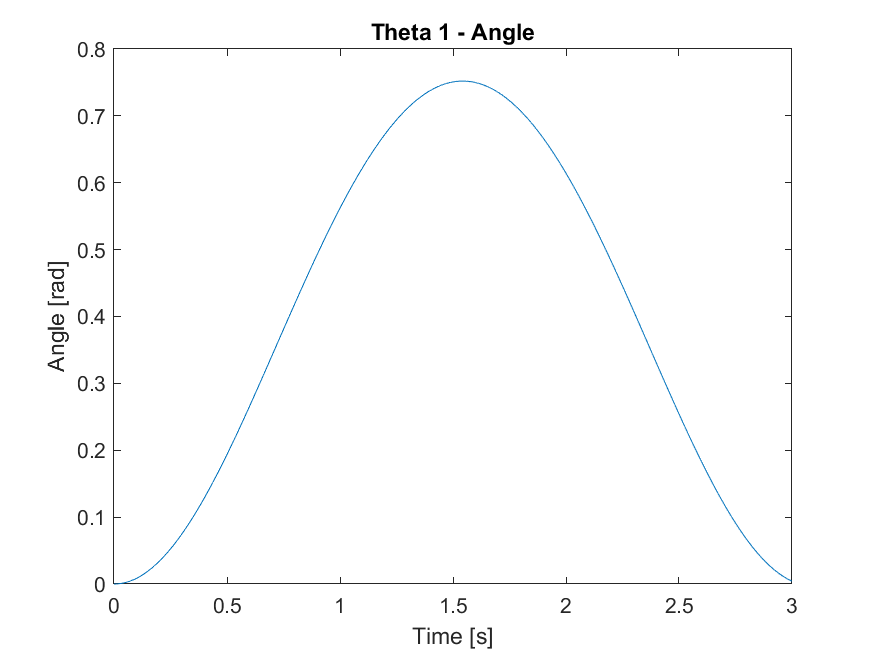
\includegraphics[scale=0.8]{graphics/Integration/theta1.png}
  \caption{Model validation of the constraint equation for body 1}
  \label{fig:Model validation of the constraint equation for body 1}
\end{figure}

Figure \ref{fig:Model validation of the constraint equation for body 1} shows the movement of the servo arm in radians, reaching its limit in one direction and returning to starting position.   

\begin{figure}[H]
  \centering
  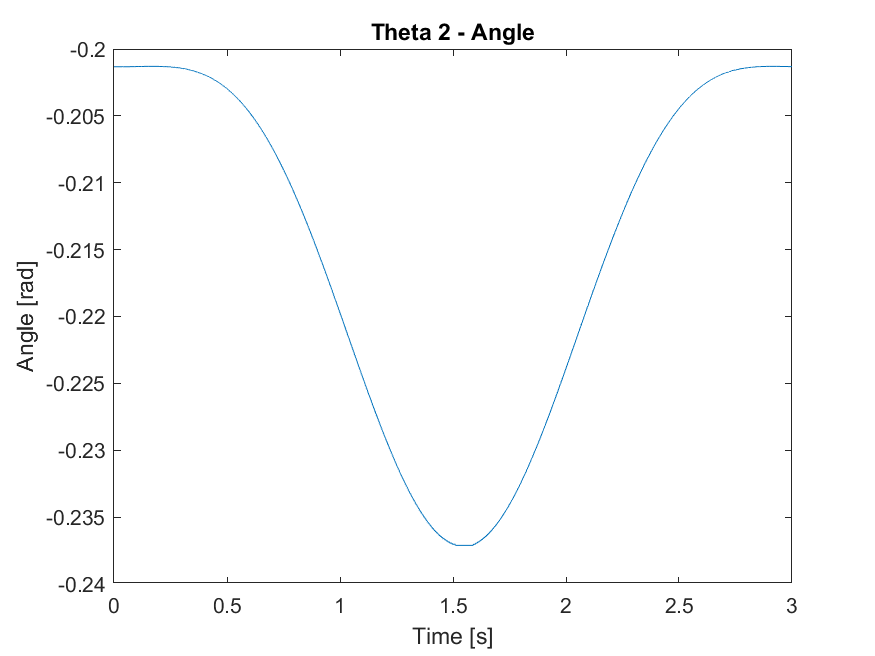
\includegraphics[scale=0.8]{graphics/Integration/theta2.png}
  \caption{Model validation of the constraint equation for body 2}
  \label{fig:Model validation of the constraint equation for body 2}
\end{figure}

Figure \ref{fig:Model validation of the constraint equation for body 2} shows the movement of the link in radians, reaching its limit in one direction and returning to starting position. The movement of the link is indeed very restrained.

\begin{figure}[H]
  \centering
  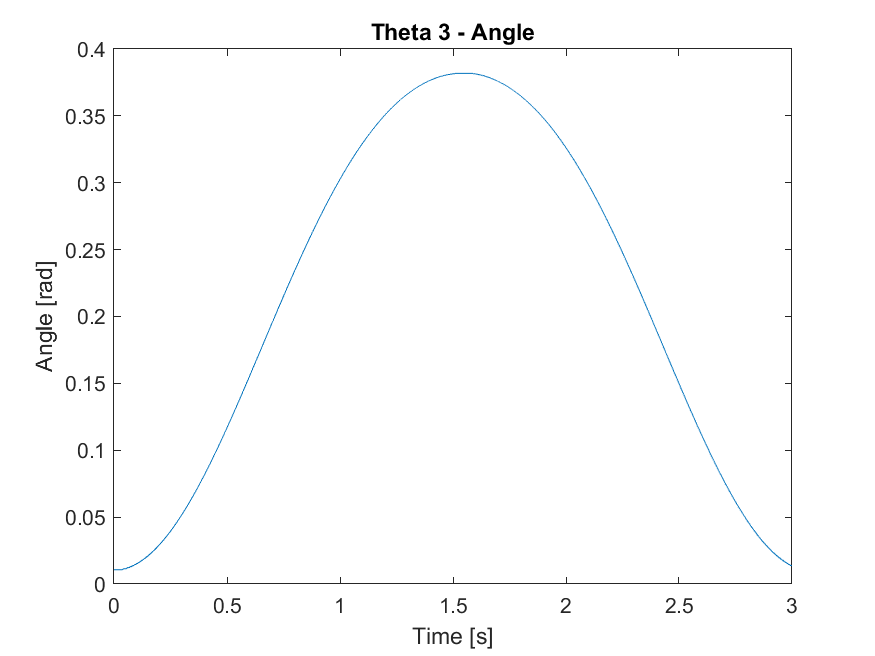
\includegraphics[scale=0.8]{graphics/Integration/theta3.png}
  \caption{Model validation of the constraint equation for body 3}
  \label{fig:Model validation of the constraint equation for body 3}
\end{figure}

Figure \ref{fig:Model validation of the constraint equation for body 3} shows the movement of the rudder in radians, reaching a limit in one direction and returning to starting position.   

The limits displayed by the simulation are consistent with the real-life behavior of the bodies, synchronized with each other. This concludes the constraint equation validation of the model. The next step in validating the model is including the UAV body into the simulation, expanding all equations to include the interactions with the other three bodies and removing all forces from the system.

Therefore, the first method of model validation was done by setting parameters to zero forces and moments to verify that it produces the expected output of zero accelerations and zero motion, with initial conditions set to equilibrium position for all bodies. 
In fig. \ref{fig:Model validation with zero forces}, Theta0 represents angular position of the UAV with respect to the inertial frame. Theta1 represents servo angle, Theta2 is the angle of the Body 2 (link between servo and rudder arm), Theta3 is the angle of the rudder. 
The model was being integrated over time, with masses and moments of inertia included but no gravitational acceleration or input force. In the case of correct model, the expected output was no motion over time. As seen in  fig.\ref{fig:Model validation with zero forces}, this was correct. 


\begin{figure}[H]
  \centering
  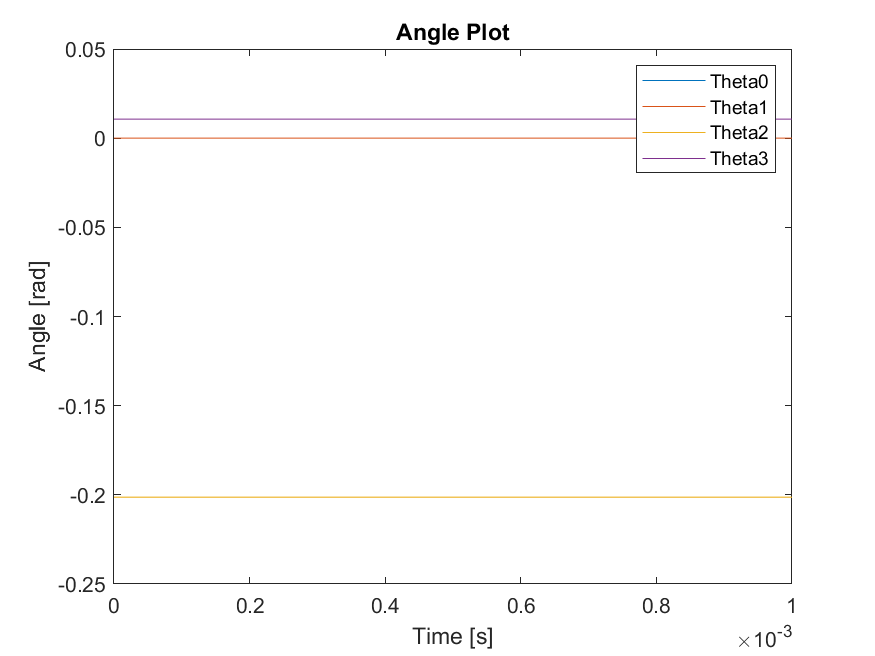
\includegraphics[scale=0.8]{graphics/Integration/staticThetas.png}
  \caption{Model validation with zero forces}
  \label{fig:Model validation with zero forces}
\end{figure}

The second test was performed by adding gravitational acceleration as the only force acting on the system, with all bodies expected to display a slow starting but accelerating movement, simulating the falling rotation of the UAV around its axis, with the other bodies attached to its frame following this motion. Fig.\ref{fig:Model validation with gravity only} shows this test, with the UAV body (Theta0) increasing its rotation about its axis unbounded. Servo (Theta1) is following UAV frame movement, without displaying its kinematic constraints specific to having had voltage input, as it does during the next test. Body 2 and Body 3 are also following the "falling" motion. 

\begin{figure}[H]
  \centering
  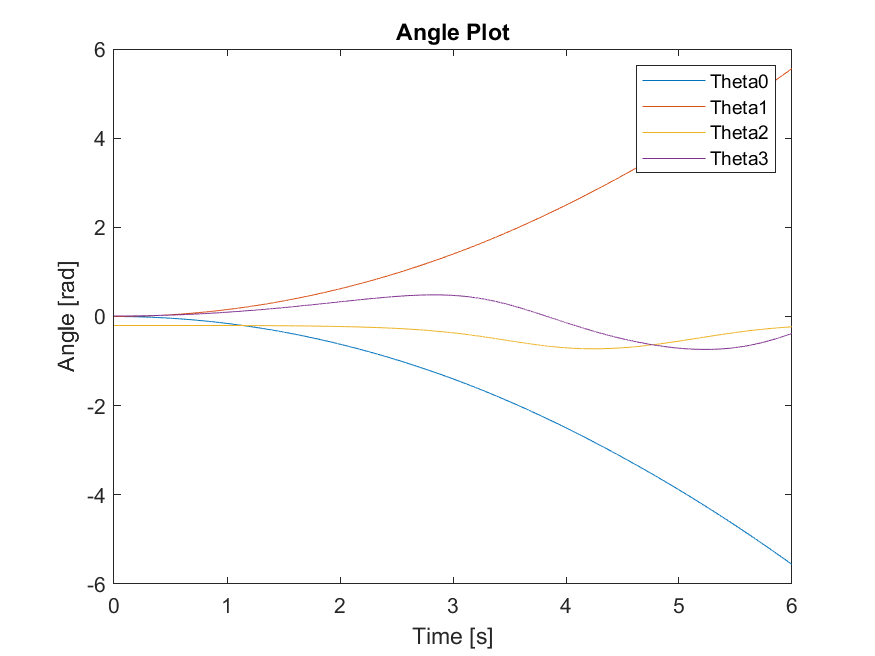
\includegraphics[scale=0.8]{graphics/Integration/g_thetas.png}
  \caption{Model validation with gravity only}
  \label{fig:Model validation with gravity only}
\end{figure}

In the third test case, the gravity parameter was kept and the propellers thrust force and servo moment were added. The expected behavior was to observe the kinematic constraints of the servo-rudder construction and the effect of the rudder on the UAV body. These are observed in fig. \ref{fig:Model validation with forces applied}, where the UAV body 0 is inclined towards an angular position of 0.4 rad, then rapidly rotating in the opposite direction, since the system is not controlled and will therefore keep tumbling. Servo (body 1) is seen to reach its kinematic limit of nearly 0.8 rad (45 degrees), moving along with the rudder (body 3) that moves in the same direction but with lower angles amplitude, to which it is rigidly linked to (body 2). 


\begin{figure}[H]
  \centering
  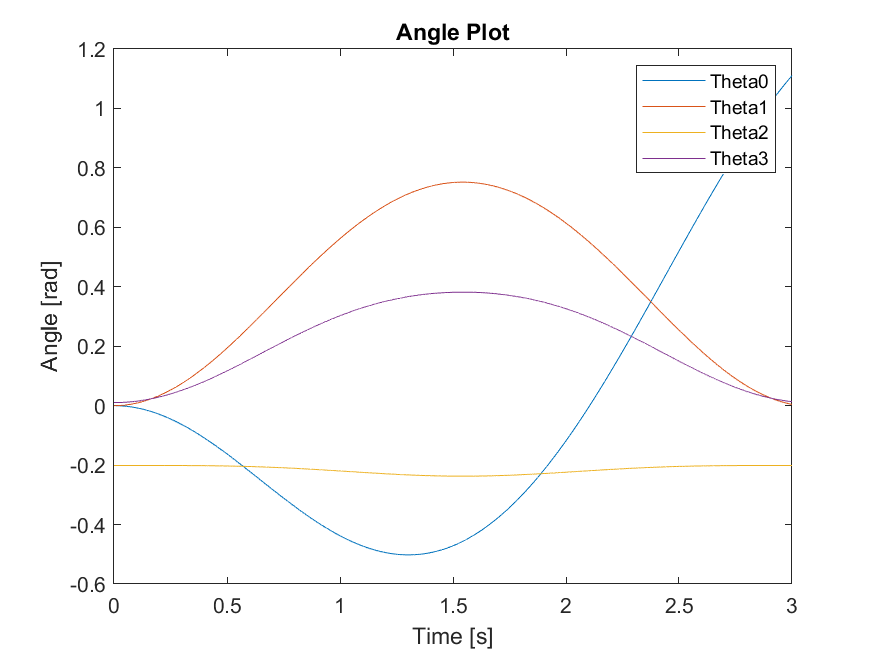
\includegraphics[scale=0.8]{graphics/Integration/thetas.png}
  \caption{Model validation with forces applied}
  \label{fig:Model validation with forces applied}
\end{figure}

Before moving into designing the controller based on the model, the model had to be correct. In this section, the model has proven to be correct. This concludes the model validation section and it can now be advanced towards the control section. 


\section{Control}

Attitude control is the process of achieving and maintaining an orientation of the rocket. 
The advantage of model based PID controller tuning is that it provides robustness with respect to sensor noise, thrust control accuracy or unmodeled plant dynamics \cite{1273571} . Likewise, having a dynamic model of the system allows for scalability, as well as tracking of system forces and their interactions. 

\textbf{Feedback control}
The feedback controller is a closed-loop servomechanism TVC system, described in the diagram below. 
The navigation system continuously updates the rocket with its current location, therefore the system knows where it is at all times; it knows this because it knows where it isn't - within reason. By subtracting where it is from where it isn't, or where it isn't from where it is (whichever is greater), it obtains a difference, or deviation. (Ground Launched Cruise Missile, 1997, p. 5) \cite{victors_1997}

The feedback controller compensates for the deviation (measured error) in order to correct the current position of the body towards the desired position (reference input point). The controller sends the signal towards the actuator, which in turn adjusts the position of the thrust vector control system, thus correcting the orientation of the plant (system). The guiding principles of this process are valid for both rocket system and UAV system. 


\begin{figure}[h!]
  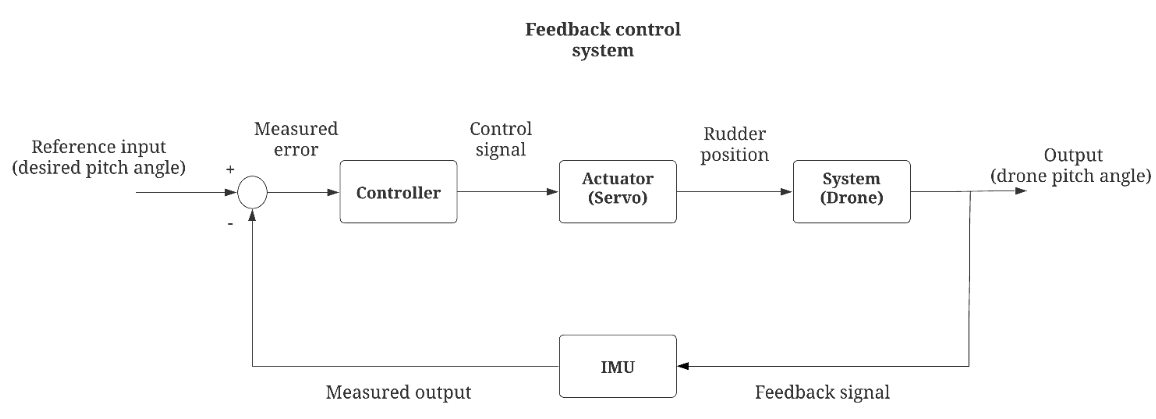
\includegraphics[scale=0.5]{graphics/Feedback.png}
  \caption{Feedback control diagram}
  \label{Feedback control diagram}
\end{figure}


The role of the controller is to minimize the error. In designing the controller, it is aimed to adjust transient and steady-state response of a control system to meet the performance requirements and adjust the parameters of the system to the desired state. \cite{yanushevsky2018modern} 

\textbf{Controller design}

In the modelling section chapter, the UAV was modeled using first principles (nonlinear physical laws).

The system has voltage to servo as input, with drone angular position as output. The thrust force of the propellers is considered part of the model as opposed to an input due to the force being a constant. 
Therefore, the system is considered a SISO (single input single output), modelled as state space model.


\textbf{Linearization }- the model obtained from first principles was highly non-linear.

While this non-linearity gives higher precision, it is resource intensive and especially so for Arduino-class micro controllers. 
Linearization  helps speed up this process and would facilitate control system design. 

This is achieved by the first order partial derivatives of the model at a steady state operating point. (Jacobian matrix)

A is the Jacobian of the function evaluated at the steady state (equilibrium position). 

\begin{flalign*}
&\text{Input equation} &\mathbf{\dot{x}}_z &= \mathbf{A}_z \mathbf{x}_z +\mathbf{B}_z \mathbf{u}_z&\nonumber\\
&\text{Output equation} &\mathbf{y}_z       &= \mathbf{C}_z \mathbf{x}_z + \mathbf{D}_z \mathbf{u}_z& 
\end{flalign*}

\begin{flalign*}
&\text{A -- System Matrix} &u\text{-Vector 1}&&\\
&\text{B -- Input Matrix } &z\text{-Vector 2}&&\\
&\text{C -- Output Matrix} &y\text{-Vector 2}&&\\
&\text{D -- Output Matrix} &                 &&
\end{flalign*}


\textbf{Linearized stability analysis}

The stability is expressed with respect to the system response as a function of time. 

In order to determine the stability of the system, its eigenvalues (poles) are analyzed, pictured in (\ref{fig:Pole-Zero Map}), Where the poles of the system are marked with an \textbf{x} and zeros are marked with \textbf{o}. It can be seen in (\ref{fig:Pole-Zero Map}) that the poles of the system have zero real part - indicating that the system is marginally stable. 

On the imaginary scale, two poles having zero imaginary parts - indicating no oscillations - and two poles placed on the axis, indicating oscillations in the system. Therefore, the purely imaginary eigenvalues describe the system as a marginally stable, undamped oscillator. 

The two zeroes of the system are placed on the real axis, at +/-0.00808. The zero in the left plane is a good solution for controller design, having stability and no oscillations. 

\begin{figure}[h!]
  \centering
  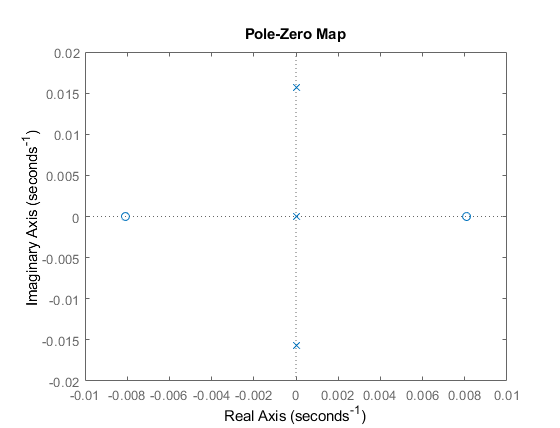
\includegraphics[scale=0.8]{graphics/PoleZeromap.png}
  \caption{Pole-Zero Map}
  \label{fig:Pole-Zero Map}
\end{figure}


The poles and zeroes are then analyzed in combination with varying gains for the feedback system, in order to determine viable solutions for the controller. The plot (\ref{fig:Root Locus Map}) shows the grid on the left hand side of the real-imaginary plane, for the values where the system is stable. 

\begin{figure}[h!]
  \centering
  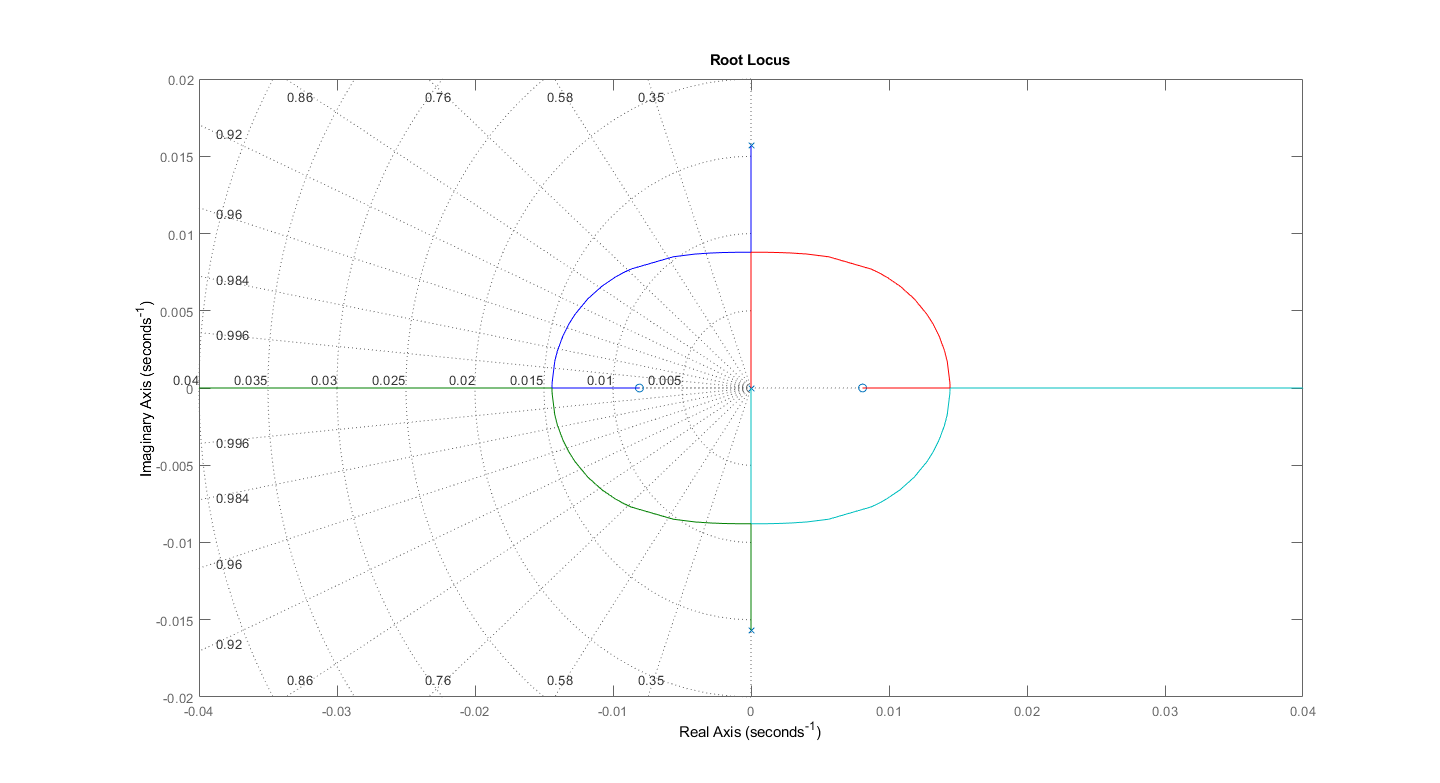
\includegraphics[scale=0.45]{graphics/rlocus.png}
  \caption{Root Locus Map}
  \label{fig:Root Locus Map}
\end{figure}


\textbf{Controllability matrix} of the state-space LTI system

Controllability is a property of a system of a particular actuator configuration to control all the states of the system; in a similar manner, observability returns the property of the particular sensor configuration to estimate all the states of the system. \cite{preumont2018vibration}

The system returns full state observability. 

Analysis of controllability matrix reveals that it has rank equal to the dimension of the state space, therefore the system is full rank controllable.

\textbf{Control}

The chosen control algorithm was a PID (Proportional Integral Derivative) controller, since literature revealed that typical control laws for rockets are variations of the PID controller. \cite{de2012spacecraft} \cite{taylor2017introduction}

An advantage of the PID is that it can fulfill the requirement of extending to additional axes because it can be decoupled - the current 1 axis control can be extended to 2 or 3 axes, which was one of the requirements. Another advantage of the PID is that a different set of gains can be calculated for different moments of inertia - in the case of the rocket, it has a different moment of inertia due to exhausting the propellants, from the moment of launch to the moment of emptying the tanks. 

The controller has a number of time-domain specifications:

\begin{itemize}
\item Rise time - time required to reach 90 percent of target
\item Maximum overshoot - exceeding target
\item Settling time - time required to reach steady state (\cite{de2012spacecraft}), page 318
\end{itemize}

The performance of the controller will be assessed against the requirements mentioned in section 1.5: max. 30 percent overshoot and 1.5 sec. settling time for the controller. 


\textbf{Simulation}

A model was prepared in Simulink for testing the control algorithm for the UAV. 

The control input is the actuator torque.

\begin{figure}[H]
    \centering
    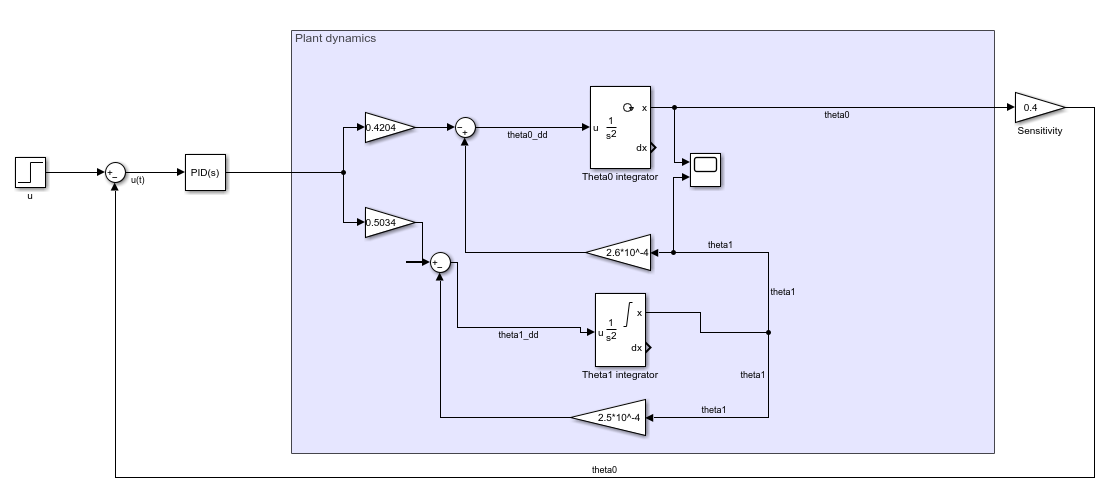
\includegraphics[scale=0.6]{graphics/Control/Simulink.png}
    \caption{Simulink model used to test PID}
     \label{Simulink Model Used to Test PID control}
\end{figure} 

The controller was initially tested with Proportional gain (kP) only, however, it was oscillating without stabilizing for any input gain. With the addition of the Derivative gain (kD), the system stabilized. The gains were tuned in order to find the set of gains which minimized overshoot, rise time and settling time of the signal. The Integral gain was found not necessary, since the system reaches reference input without any significant steady state error to be corrected for - and the Integral (kI) gain was found to be otherwise detrimental to the performance, introducing overshoot, oscillation and increasing the settling time, as well as the potential of wind-up - and was therefore set to 0. 

In the Simulink model, the initial condition for UAV angular position was set to 0.2 rad, corresponding to a starting inclination that the controller will have to correct for in order to reach angular position of 0 rad. The velocity of the UAV was set to 0.2 rad/s initial condition. With these conditions, the best performing set of gains was found to be kP = -2 and kD = -8.  

\begin{figure}[H]
    \centering
    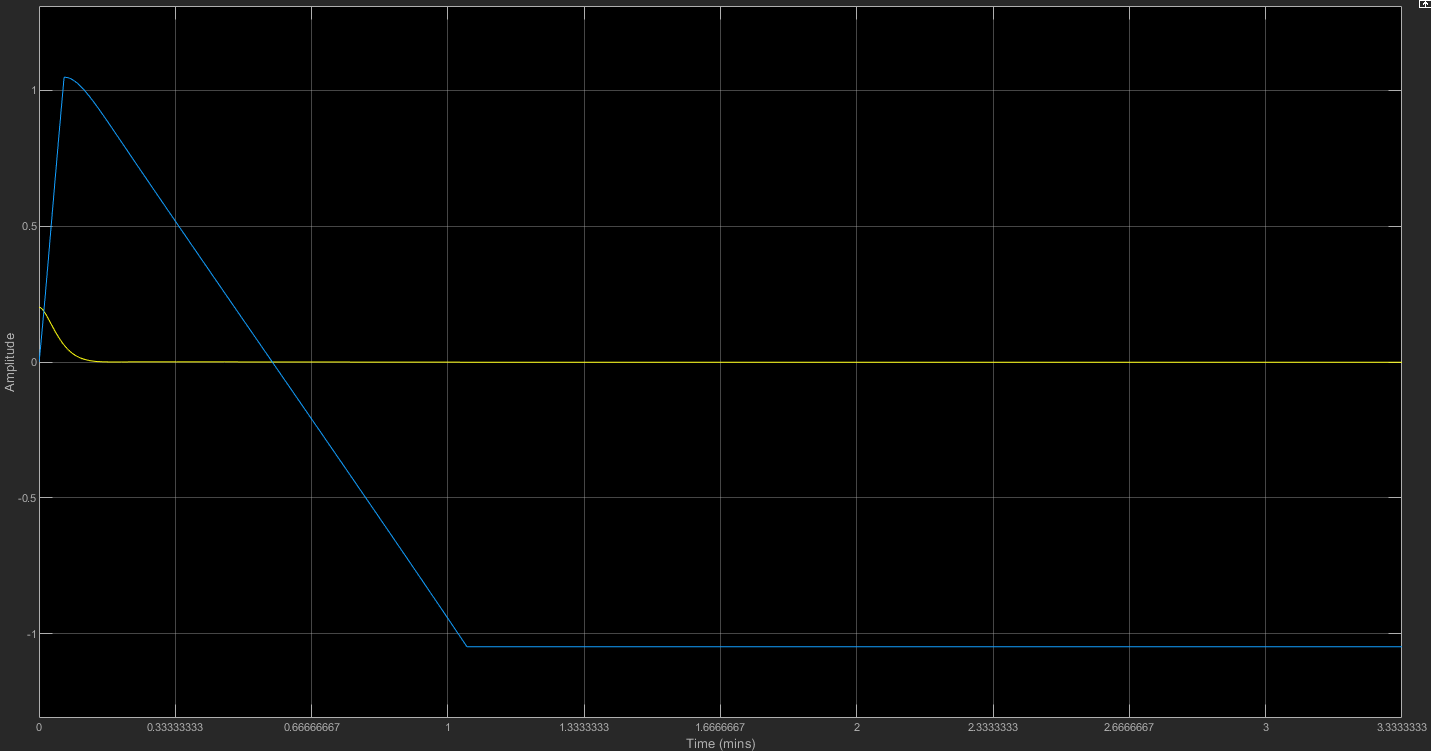
\includegraphics[scale=0.3]{graphics/Control/TSP2D6.png}
    \caption{Oscilloscope graph of the angular position of UAV and servo angle}
     \label{fig:Oscilloscope graph of the angular position of UAV and servo angle}
\end{figure} 

In \ref{fig:Oscilloscope graph of the angular position of UAV and servo angle}, theta0 represents the angular position of the UAV and theta1 represents the servo (actuator) position. With the mentioned gains, the system was found to have no overshoot, no necessary rising time and a settling time of 0.2 seconds. The controller thus sets the system, a harmonic oscillator, into a critically damped oscillator, reaching the equilibrium position of 0 rad quickly with no overshoot or oscillations. With this controller, the system remains critically damped with any initial condition ranging from 0 to +-0.8 radians (45 degrees)
This fulfills the requirements of having under 30 percent overshoot and under 1.5 settling time. 



\textit{This chapter discussed the modelling and control decisions for the project, approaches which are to be demonstrated in the following chapter in tests. }

